\documentclass{article}

% if you need to pass options to natbib, use, e.g.:
%     \PassOptionsToPackage{numbers, compress}{natbib}
% before loading neurips_2024


% ready for submission
\usepackage[final, accepted]{neurips_2024}


% to compile a preprint version, e.g., for submission to arXiv, add add the
% [preprint] option:
%     \usepackage[preprint]{neurips_2024}


% to compile a camera-ready version, add the [final] option, e.g.:
%     \usepackage[final]{neurips_2024}


% to avoid loading the natbib package, add option nonatbib:
%    \usepackage[nonatbib]{neurips_2024}


\usepackage[utf8]{inputenc} % allow utf-8 input
\usepackage[T1]{fontenc}    % use 8-bit T1 fonts
\usepackage{hyperref}       % hyperlinks
\usepackage{url}            % simple URL typesetting
\usepackage{booktabs}       % professional-quality tables
\usepackage{amsfonts}       % blackboard math symbols
\usepackage{nicefrac}       % compact symbols for 1/2, etc.
\usepackage{microtype}      % microtypography
\usepackage{xcolor}         % colors
\usepackage{subfigure}  % Add this in preamble
\usepackage{graphicx}  % Add this in preamble
\usepackage{float}  % Add this with your other packages at the top
\usepackage{amsmath}
\usepackage{natbib}
\usepackage{hyperref}


\title{
   \Large Regression of Used Car Prices \\[4mm]
   \normalsize AI6102-GroupA-Machine Learning Methodologies \& Applications \\[2mm]
   \normalsize Kaggle Challenge \\[2mm]
}


% The \author macro works with any number of authors. There are two commands
% used to separate the names and addresses of multiple authors: \And and \AND.
%
% Using \And between authors leaves it to LaTeX to determine where to break the
% lines. Using \AND forces a line break at that point. So, if LaTeX puts 3 of 4
% authors names on the first line, and the last on the second line, try using
% \AND instead of \And before the third author name.


\author{
    Eugene Ho Hong Zhuang\\
    G2204889B\\
    Nanyang Technological University\\
    \texttt{eho010@e.ntu.edu.sg}\\
    \And
    Teixayavong SalineLat\\
    G2303887A\\
    Nanyang Technological University\\
    \texttt{salinela001@e.ntu.edu.sg}\\
    \And
    Pan Feng\\
    G2405221K\\
    Nanyang Technological University\\
    \texttt{feng006@e.ntu.edu.sg}\\
    \\[\baselineskip]  % Add extra space before GitHub link
    \hfill\url{https://github.com/genehhz/AI6102---Machine-Learning-Methodologies-Applications}\hfill\mbox{}  % Center with some indent
}


\begin{document}


\maketitle


\begin{abstract}
This study explores the application of machine learning algorithms to predict used car resale prices using a dataset of 188,533 vehicles with 13 features. The research involved extensive data preprocessing, including handling missing values, feature extraction from unstructured text descriptions of engine and transmission specifications, and recategorization of color variables. Six machine learning models were developed and compared: Ridge Regression, LightGBM, XGBoost, CatBoost, Multi-Layer Perceptron, and Gaussian Na\"{i}ve Bayes. Using 5-fold cross-validation and root mean squared error (RMSE) as the evaluation metric, LightGBM emerged as the best-performing model with a test RMSE of 63,481.83, significantly outperforming the baseline Ridge Regression, RMSE: 64,743.27.
\end{abstract}


\section{Introduction}

The automotive resale market plays a crucial role in the economy, with buyers and sellers relying on accurate price predictions to make informed decisions. Predicting the resale value of used cars is a challenging problem due to the interplay of multiple factors, including vehicle specifications, market trends, and consumer preferences. This report explores the application of machine learning techniques to predict the resale price of used cars based on various features. The primary goal is to build a robust predictive model that can aid stakeholders in estimating the resale value in unseen data instances with high accuracy.

\section{Dataset, Attributes and Outcome}

The dataset used in this study is obtained from a Kaggle competition~\cite{playground-series-s4e9} focused on predicting the resale price of used cars. The dataset was synthetically generated, but it still provides a rich collection of features that comprehensively describe the vehicles and their conditions, along with the target variable, \textit{price}. The dataset includes both numerical and categorical attributes, offering a balanced mix of quantitative and qualitative information. This structure allows for an in-depth exploration of feature interactions and an evaluation of the effectiveness of machine learning models for supervised-learning for regression prediction.

The dataset is divided into training and test sets. The training dataset, containing \textbf{188,533 rows and 13 features}, includes the target variable \textit{price}, making it suitable for supervised model training. In contrast, the test dataset comprises \textbf{125,690 rows and 12 features}, excluding the target variable, and is used for evaluating model performance on unseen data. The full list of variables includes \texttt{id}, \texttt{brand}, \texttt{model}, \texttt{model\_year}, \texttt{milage}, \texttt{fuel\_type}, \texttt{engine}, \texttt{transmission}, \texttt{ext\_col}, \texttt{int\_col}, \texttt{accident}, \texttt{clean\_title}, and \texttt{price}. These variables represent a broad spectrum of car attributes, from technical specifications to ownership history.

The dataset consists of both numerical and categorical attributes, offering a mix of quantitative and qualitative information:

\begin{itemize}
   \item \textbf{Numerical Features}: \texttt{model\_year} and \texttt{milage}
   
   \item \textbf{Categorical Features}: \texttt{id}, \texttt{brand}, \texttt{model}, \texttt{fuel\_type}, \texttt{engine}, \texttt{transmission}, \texttt{ext\_col}, \texttt{int\_col}, \texttt{accident}, and \texttt{clean\_title}
   
   \item \textbf{Target Variable}: The target variable, \texttt{price}, is a continuous numerical variable representing the predicted resale value
\end{itemize}

The dataset offers an excellent opportunity to explore feature interactions and evaluate the effectiveness of machine learning models in a real-world regression problem.

\section{Data Preprocessing}

\subsection{Missing or Null Values}

In both the training and test sets, only three variables had missing values: \texttt{fuel\_type}, \texttt{accident} and \texttt{clean\_title}. The missing value rates were 1.3\% for \texttt{accident}, 2.7\% for \texttt{fuel\_type} and 11.4\% for \texttt{clean\_title} in both the training and test sets.

Missing values in these variables were addressed using imputation techniques. For the \texttt{clean\_title} variable, missing entries were filled with the value `no', indicating the absence of a clean title. Similarly, the \texttt{accident} variable was imputed with the value `None reported' for missing rows. Missing values for the \texttt{fuel\_type} variable cannot be simply inferred, we employed additional steps to address missing values for this variable. We first extracted information on fuel type embedded within the \texttt{engine} variable. Any remaining unfilled missing values are imputed using the mode fuel type of the corresponding car brand.

\begin{figure}[H]
   \centering
   \begin{minipage}[b]{0.45\textwidth}
       \centering
       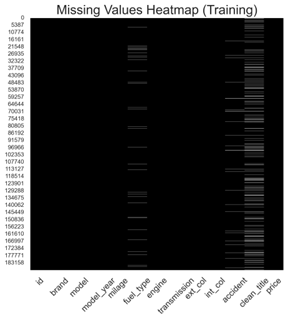
\includegraphics[width=\textwidth]{heatmap1.png}
       \centerline{(A)}
   \end{minipage}
   \hfill
   \begin{minipage}[b]{0.45\textwidth}
       \centering
       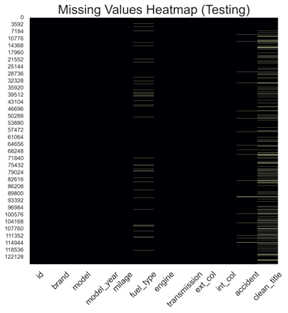
\includegraphics[width=\textwidth]{heatmap2.png}
       \centerline{(B)} 
   \end{minipage}
   \caption{Heatmap illustrating the missing values in training (A) and test (B) set}
   \label{fig:heatmaps}
\end{figure}

\subsection{Features Extractions and Imputations}

The columns \texttt{engine} and \texttt{transmission} contain long texts for the detailed descriptions of the vehicle's engine specifications and attributes related to the gearbox and its functionality. Texts within \texttt{engine} and \texttt{transmission} were parsed and extracted for both the training (df) and test (dt) datasets to ensure that these descriptions were meaningful, structured and machine-readable, facilitating improved predictive modeling and analysis. Details extracted from \texttt{engine} were stored in new columns: \texttt{engine\_hp}, \texttt{engine\_liter}, \texttt{engine\_cyl}, and \texttt{engine\_fuel}.

\begin{enumerate}
   \item \textbf{Horsepower (\texttt{engine\_hp})}: The numeric horsepower value was identified using a regular expression that matches patterns such as 250 hp. Missing values were imputed with NaN.
   
   \item \textbf{Engine Capacity in Liters (\texttt{engine\_liter})}: Liter specifications, e.g., 2.0L, were extracted using a regular expression and converted to numeric values. Missing entries were also imputed with NaN.
   \begin{enumerate}
       \item NaN was eventually imputed with median value
   \end{enumerate}
   
   \item \textbf{Number of Cylinders (\texttt{engine\_cyl})}: Cylinder counts were derived from patterns like 4 cylinders or Roman numerals (e.g., IV cylinders). These were converted to integers or left as NaN for missing values.
   \begin{enumerate}
       \item NaN was eventually imputed with median value
   \end{enumerate}
   
   \item \textbf{Fuel Type (\texttt{engine\_fuel})}: Fuel types such as Gasoline, Diesel, Electric, Hybrid, E85 Flex Fuel, and Plug-In Hybrid were identified from a predefined list of options. If no match was found, the value was set to NaN. Electric and Hybrid were manually imputed using the following rules:
   \begin{enumerate}
       \item Electric was imputed for cars that are from electric vehicles-based brands, including Tesla, Rivian, Lucid, and Polestar.
       \item Hybrid was imputed for cars with imputed cars with imputed Electric but also showed engine capacity.
   \end{enumerate}
\end{enumerate}

Key extracted features from \texttt{transmission} include:

\begin{enumerate}
   \item \textbf{Number of Gears (\texttt{gears})}: Patterns like 6-speed or 6 speed were parsed to extract the number of gears as integers. Special cases like single-speed were normalized to 1. Missing values were left as None.
   
   \item \textbf{Transmission Type (\texttt{transmission\_type})}: Transmission types were categorized into values such as Automatic, Manual, CVT, AMT, Dual\_Shift and Electronically\_controlled.
   
   \item \textbf{Special Features (\texttt{special\_features})}: Additional transmission features like Dual Shift Mode, Auto-Shift, Overdrive, Variable, and Electronically Controlled were identified and recorded. Missing values were left as 'missing', pertaining to not applicable.
   
   \item \textbf{Transmission Designation (\texttt{transmission\_designation})}: Common transmission abbreviations such as A/T, M/T, DCT, and CVT were extracted to create a standard designation field. Missing values were left as 'missing', pertaining to not applicable.
\end{enumerate}

\subsection{Other transformation and Encoding}
\subsubsection{Recategorizing Interior and Exterior Car Colour}
The \texttt{ext\_col} (exterior color) and \texttt{int\_col} (interior color) variables were pre-processed by grouping specific hues or tones into broader base color categories. This step reduced the complexity of analyzing the wide variety of descriptive color names in the dataset. We matched the text of the original color description to any entries within a predefined list of base colors: [\texttt{'white'}, \texttt{'black'}, \texttt{'grey'}, \texttt{'gray'}, \texttt{'blue'}, \texttt{'red'}, \texttt{'yellow'}, \texttt{'silver'}, \texttt{'green'}, \texttt{'beige'}, \texttt{'gold'}, \texttt{'orange'}, \texttt{'brown'}, \texttt{'ebony'}, \texttt{'purple'}]. If a match was found, the function returned the corresponding base color. If no match was identified, the value was categorized as ``uncommon'' to capture rare or non-standard colors.

\subsubsection{Creating and Dropping Variables}

\begin{itemize}
   \item The variable \texttt{model\_year} was converted into \texttt{Vehicle\_Age} by substituting it from current year (2024)

   \item The binary variable \texttt{Is\_Luxury\_Brand} was created. Cars were deemed to be luxuries if their brands were either ``mercedes-benz'', ``bmw'', ``audi'', ``porsche'', ``lexus'', ``cadillac'', ``jaguar'', ``bentley'', ``genesis'', ``maserati'', ``lamborghini'', ``rolls-royce'', ``ferrari'', ``mclaren'', ``aston'', ``lotus'', ``bugatti'', or ``maybach''.

   \item Variables that were dropped include \texttt{id}, \texttt{model}, \texttt{transmission}, \texttt{engine}, \texttt{engine\_fuel}, and \texttt{model\_year}.
\end{itemize}

\subsubsection{One-hot encoding of categorical variables}

\begin{itemize}
   \item The OneHotEncoder function from sklearn (preprocessing) was applied on categorical variables to one-hot encode them, making them more amenable as inputs into models.
   
   \item The seven final categorical variables and their levels are:
\end{itemize}
\begin{table}[h]
   \centering
   \caption{Categorical variable and their corresponding levels}
   \label{tab:categorical_vars}
   \begin{tabular}{ll}
       \hline
       Variable & Levels \\
       \hline
       \texttt{brand} & 57 \\
       \texttt{fuel\_type} & 6 \\
       \texttt{ext\_col} & 15 \\
       \texttt{int\_col} & 14 \\
       \texttt{clean\_title} & 2 \\
       \texttt{transmission\_type} & 9 \\
       \texttt{Special\_features} & 6 \\
       \hline
   \end{tabular}
\end{table}

The full list of features and their details after preprocessing can be seen in Appendix Table A.1. 
\newpage
\section{Exploratory Data Analysis (EDA) and Visualisation}

EDA was conducted to uncover underlying patterns, relationships, and anomalies in the dataset. Both univariate and multivariate visualizations were employed to understand the distribution of individual features and their interactions with the target variable. Insights from EDA were instrumental in shaping feature selection and subsequent model design.

\subsection{Continuous Variables}
\subsubsection{Price Distribution}

From the distribution plots above, we can see that resale price is highly skewed (right-skewed), with 94\% of cars priced under \$100,000. Car prices ranged from \$2,000 -- \$2,954,083.

\begin{figure}[H]
    \centering
    \begin{minipage}[b]{0.45\textwidth}
        \centering
        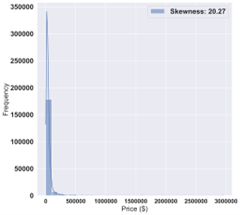
\includegraphics[width=\textwidth]{frequency_price.png}
        \centerline{(A)}
    \end{minipage}
    \hfill
    \begin{minipage}[b]{0.45\textwidth}
        \centering
        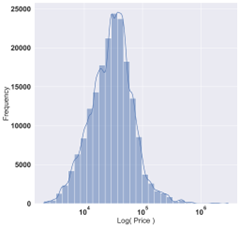
\includegraphics[width=\textwidth]{frequency_logprice.png}
        \centerline{(B)}
    \end{minipage}
    \caption{(A) Frequency distribution of mileage, (B) Scatterplot of Price against Mileages}
    \label{fig:mileage_dist}
\end{figure}

\subsubsection{Mileage Distribution}

Mileage distribution is acceptable, and shows a negative relationship with car prices (i.e., cars with higher mileages have lower prices).

\begin{figure}[H]    % Using [H] for strict "Here" placement
    \centering
    \begin{minipage}[b]{0.45\textwidth}
        \centering
        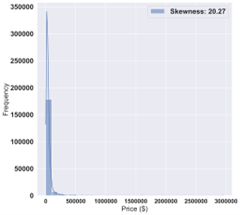
\includegraphics[width=\textwidth]{frequency_price.png}
        \centerline{(A)}
    \end{minipage}
    \hfill
    \begin{minipage}[b]{0.45\textwidth}
        \centering
        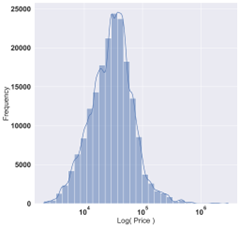
\includegraphics[width=\textwidth]{frequency_logprice.png}
        \centerline{(B)}
    \end{minipage}
    \caption{Frequency distribution of price (A) and log(price) (B)}
    \label{fig:price_dist}
\end{figure}

\subsubsection{Age of Vehicle Distribution}

Vehicle age distribution is acceptable, and shows a weak negative relationship with car prices.

\begin{figure}[H]    % Using [H] for strict "Here" placement
   \centering
   \begin{minipage}[b]{0.45\textwidth}
       \centering
       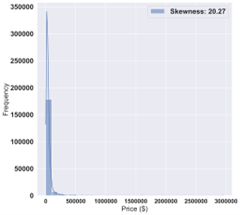
\includegraphics[width=\textwidth]{image5.png}
       \centerline{(A)}
   \end{minipage}
   \hfill
   \begin{minipage}[b]{0.45\textwidth}
       \centering
       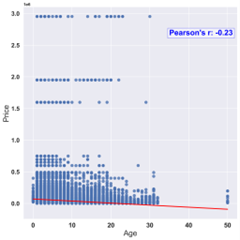
\includegraphics[width=\textwidth,height=0.9\textwidth]{image6.png}  % Added height parameter
       \centerline{(B)}
   \end{minipage}
   \caption{(A) Frequency distribution of vehicle Age, (B) Scatterplot of Price against Age with pearson correlation coefficient of these 2 variables}
   \label{fig:price_dist}
\end{figure}

\subsection{Categorical Variables}
\subsubsection{Car Brands}

Five most common car brands include Ford, Mercedes-Benz, BMW, Chevrolet, and Audi, and they are priced in mid- to upper-range in terms of average car prices. Brands with the highest resale values were Bugatti, Lambhorgini, Rolls-Royce, Bentley, and McLaren, reselling at more \$120,000 on average. On the other hand, brands with the lowest resale values included Scion, Hammer, Mini, Saturn, and Mitsubishi, reselling at \$20,000 or less on average. Expectedly, brands carried great significance in the resale values of cars.

\begin{figure}[H]
   \centering
   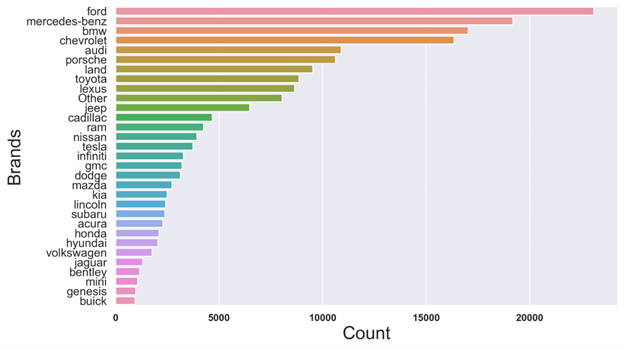
\includegraphics[width=0.8\textwidth]{image7.png}  % Adjust width as needed
   \caption{Frequency distribution of car brands by count}
   \label{fig:brand_dist}
\end{figure}

\begin{figure}[H]
   \centering
   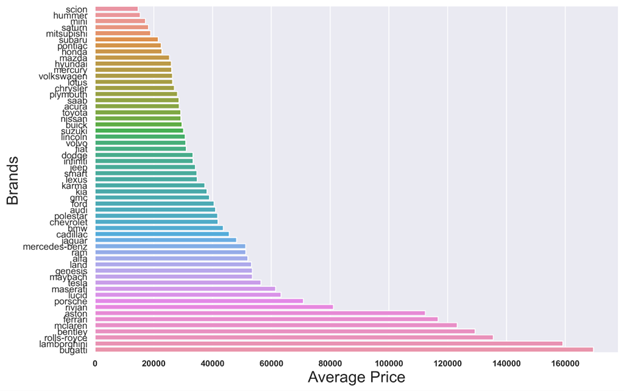
\includegraphics[width=0.8\textwidth]{image8.png}  % Adjust width as needed
   \caption{Average price for each car brands}
   \label{fig:brand_dist}
\end{figure}

\subsubsection{Fuel Types}

The most prevalent fuel types in the dataset was gasoline (88\%), indicating that the feature shows marked skewness. Fuel types seem to also affect the average resale prices, with all-electric and hybrid cars having the two highest resale values (\$50,000) while gasoline (\$43,308) and flex-fuel cars (\$26,698) had the lowest average resale values.

\begin{figure}[H]    % Using [H] for strict "Here" placement
   \centering
   \begin{minipage}[b]{0.45\textwidth}
       \centering
       \includegraphics[width=\textwidth]{image9.png}
       \centerline{(A)}
   \end{minipage}
   \hfill
   \begin{minipage}[b]{0.45\textwidth}
       \centering
       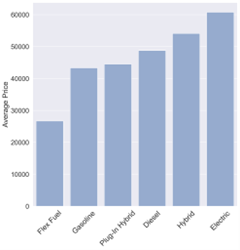
\includegraphics[width=\textwidth,height=0.9\textwidth]{image10.png}  % Added height parameter
       \centerline{(B)}
   \end{minipage}
   \caption{(A) Frequency distribution of fuel types by count, (B) Average price of different fuel types}
   \label{fig:price_dist}
\end{figure}

\subsubsection{Color Popularity and Price}

The most common exterior car colors were black, white, gray, and silver (all $>$10\% of all car colors). Though, among these, only gray and black cars had higher than average resale values. Other colors that managed to receive good resale prices included uncommon colors, green, orange, and yellow.

There was also significant variability in interior colors and their relationships with resale price. Black was by far the most common interior color (59\% of all cars), and had higher than average resale price. Beige and gray were other two common interior colors, but they did not have a high resale price. Interestingly, yellow interior, a rare interior color, had an unusually high resale value at \$106,548.

\begin{figure}[H]
   \centering
   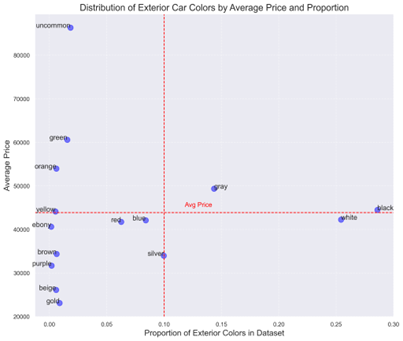
\includegraphics[width=0.8\textwidth]{image12.png}  % Adjust width as needed
   \caption{Scatterplot of Average Price against Exterior Colours}
   \label{fig:brand_dist}
\end{figure}

\begin{figure}[H]
   \centering
   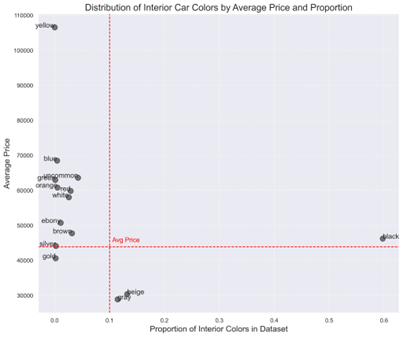
\includegraphics[width=0.8\textwidth]{image13.png}  % Adjust width as needed
   \caption{Scatterplot of Average Price against Interior Colors}
   \label{fig:brand_dist}
\end{figure}

\subsubsection{Engine and Transmission Configurations}

From Figure~10, there is moderate skewness for \texttt{engine\_hp} and \texttt{engine\_liter}, and weak relationship with price.

\begin{figure}[H]
   \centering
   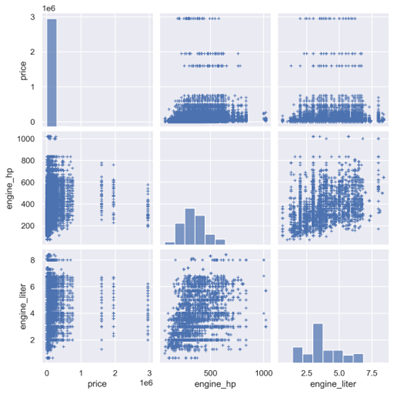
\includegraphics[width=0.8\textwidth]{image14.png}  % Adjust width as needed
   \caption{Pairplot illustrating the correlations of multi-variable - \texttt{price}, \texttt{engine\_hp} and \texttt{engine\_litre}}
   \label{fig:brand_dist}
\end{figure}

\newpage
From Figure~11, for both \texttt{gears} and \texttt{transmission\_types}, median car price did not vary across categories. However, the median price seemed to be higher for transmission with Auto-Shift feature. Price also seemed to increase with the number of engine cylinders. Across all categories of each feature, there are outlier prices to suggest skewed distributions.

\begin{figure}[H]
   \centering
   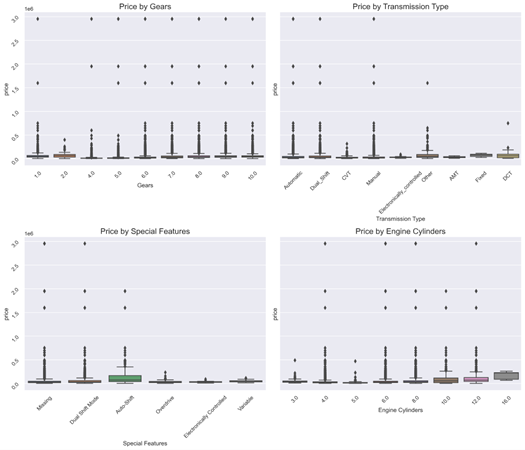
\includegraphics[width=0.8\textwidth]{image15.png}  % Adjust width as needed
   \caption{Boxplots of price against different variables: gears, transmission type, special features and engine cylinders}
   \label{fig:brand_dist}
\end{figure}

\subsubsection{Other Variables}

The history of reported accidents also significantly impacts a car's resale price. Vehicles with a reported history of accidents generally exhibit lower average prices compared to those with no accidents. For instance, cars with a clean accident history have an average price of \textbf{\$49,122}, while those with a reported accident history are priced around \textbf{\$25,334}. This difference reflects buyer preferences for cars perceived as more reliable and in better condition, emphasizing the importance of accident-free histories in the used car market.

A car's title status is a critical factor in determining its resale value. Vehicles with a clean title, indicating no major damage, theft, or salvage history, command higher prices than those without. The analysis reveals that cars with clean titles have an average price of \textbf{\$63,567}, whereas cars with branded or salvage titles average around \textbf{\$41,354}. This stark difference highlights the significant role of title status in buyer confidence and perceived vehicle quality.

The distinction between luxury and non-luxury brands is a pivotal variable influencing car prices. Luxury brands, such as Mercedes, BMW, and Lexus, maintain higher average prices due to their brand reputation, premium features, and perceived status. The analysis shows that luxury brands have an average price of \textbf{\$52,368}, compared to \textbf{\$37,929} for non-luxury brands. This disparity underscores the enduring demand and value retention of luxury vehicles in the resale market.
\newpage
\section{Model Development}

We employed a variety of machine learning algorithms, ranging from simple classical models to more complex architectures, to predict car prices. The prediction task involves supervised regression problem, where the goal was to estimate the target variable, \texttt{price}, for unseen test instances. By employing models of varying complexity, we aimed to evaluate how incremental increases in model sophistication improved predictive performance on both the validation and test sets. As the baseline, we used linear regression with L2 regularization (i.e., ridge regression), a simple yet effective algorithm. This approach allowed us to model linear relationships within the data and served as a benchmark to understand the added value of more complex algorithms. Ridge regression provided a clear starting point for interpreting how regularization controls overfitting while retaining simplicity and computational efficiency.

Building on this, we incorporated three advanced gradient-boosting models ~\cite{4a848dd1-54e3-3c3c-83c3-04977ded2e71}: LightGBM ~\cite{NIPS2017_6449f44a}, XGBoost~\cite{10.1145/2939672.2939785}, and CatBoost~\cite{10.5555/3327757.3327770}. These algorithms are highly adept at capturing non-linear relationships in the data and are particularly effective in handling large numbers of features, including categorical variables. Their ability to perform efficient feature selection and mitigate overfitting through ensemble techniques ensure optimal performance.

Next, we evaluated the performance of a Multi-Layer Perceptron (MLP) ~\cite{10.5555/1639537.1639542}, a fundamental deep learning architecture. Unlike tree-based models, MLPs excel at learning complex, non-linear interactions between features through their multi-layered structure of fully connected neurons. This made the MLP a valuable addition to our study, particularly for exploring intricate patterns in high-dimensional data.

Lastly, we assessed the Na\"{i}ve Bayes classifier for its probabilistic approach to modeling categorical data ~\cite{8947658}. While traditionally used for classification tasks, its application in this study offered a unique perspective on how simple probabilistic assumptions could capture the relationships in categorical features and contribute to the overall predictive task. Below, we provide detailed descriptions of each model used in our analysis.

\subsection{Training Procedure and Model Selection}

The training of each model adheres to a consistent 5-fold cross-validation (CV) strategy to ensure robust performance evaluation ~\cite{wong2019reliable}. In this approach, the dataset is divided into five equal-sized folds. During each iteration, four folds are used for training while the remaining fold serves as the validation set. This process is repeated five times, ensuring that every fold is used as a validation set exactly once. The average Root Mean Squared Error (RMSE) across the five validation folds is computed to evaluate the model's performance during training and hyperparameter tuning.

After the cross-validation process, each model is further evaluated on a held-out test set to calculate the test RMSE. This ensures that the model's performance is assessed on entirely unseen data, providing a reliable estimate of its generalization capability. For the final stage, the model with the best validation RMSE is re-trained on the entire training dataset (excluding the test set) to fully utilize all available data. This re-trained model is then used to generate final predictions on the test set, and the resulting RMSE is recorded as the model's definitive performance metric. The consistency in training methodology across the Ridge Regression, LightGBM, XGBoost, CatBoost, and MLP models ensures fair comparisons, while the comprehensive use of CV and test evaluation provides a thorough assessment of each model's predictive capability.

\subsection{Performance Metric}

In this Kaggle challenge, the scores are evaluated based on the Root Mean Square Error (RMSE) between predicted price and original price as seen in the equation below. Hence, RMSE was employed to evaluate model performance across training, validation, and testing phases, providing a consistent metric for assessing prediction accuracy.

\begin{equation}
   RMSE = \left(\frac{1}{N}\sum_{i=1}^{N}(y_i - \hat{y}_i)^2\right)^{1/2}
\end{equation}

\subsection{Machine Learning Models}
\subsubsection{Ridge Regression with L2 Regularisation}

Ridge regression was chosen as the baseline model due to its simplicity and interpretability. This algorithm extends linear regression by incorporating L2 regularization, which penalizes large coefficients to mitigate overfitting. The regularization strength is controlled by the hyperparameter $\lambda$, where a larger $\lambda$ results in stronger penalization, and a smaller $\lambda$ approaches standard linear regression. After fine-tuning, an optimal $\lambda$ of 0.5 was adopted. The parameters (i.e., weights) of the model were computed using the analytical closed-form solution (using sklearn's \texttt{LinearRegression}) rather than iterative gradient descent.

\subsubsection{LightGBM (LGBM)}

LightGBM employs gradient boosting with a leaf-wise tree growth strategy, expanding the leaf that maximizes the reduction in loss at each step. This minimizes the objective function:

\begin{equation}
    L(\Theta) = \sum_{i=1}^n \ell(y_i, \hat{y}_i) + \lambda \sum_{j=1}^T \|w_j\|^2
\end{equation}

where $\ell(y_i, \hat{y}_i)$ is the loss (e.g., root mean squared error), $w_j$ are the leaf weights, $T$ is the number of leaves, and $\lambda$ is the regularization term.

LightGBM optimizes using histogram-based binning to accelerate split finding and uses Gradient-Based One-Side Sampling (GOSS) to retain instances with larger gradients, ensuring effective learning while reducing data size. Exclusive Feature Bundling (EFB) combines sparse features into a single feature, reducing dimensionality without loss of information. LightGBM's efficiency stems from these optimizations, enabling fast training on large datasets.

To further optimize the model, we mainly experimentally tuned \texttt{num\_leaves}, \texttt{max\_depth}, \texttt{learning\_rate}, \texttt{min\_data\_in\_leaf}, \texttt{feature\_fraction}, \texttt{bagging\_fraction} and \texttt{bagging\_freq} as these parameters impact the model the most. As can seen from the photo below, different versions of lightgbm model were submitted, and the RMSE score increased from 63542.09 (version 1) to 6348.83 (version 3) after tuning the above mentioned parameters.

\begin{table}[h]
    \centering
    \caption{Final hyperparameters used for LightGBM}
    \begin{tabular}{ll}
        \hline
        \textbf{Hyperparameters} & \textbf{Value} \\
        \hline
        num\_leaves & 150 \\
        max\_depth & 15 \\
        learning\_rate & 0.02 \\
        n\_estimators & 1000 \\
        metric & RMSE \\
        subsample & 0.6 \\
        colsample\_bytree & 0.9 \\
        reg\_alpha & 0.2 \\
        reg\_lambda & 1 \\
        objective & regression \\
        min\_data\_in\_leaf & 350 \\
        feature\_fraction & 0.75 \\
        bagging\_fraction & 0.6 \\
        bagging\_freq & 2 \\
        random\_state & 42 \\
        min\_child\_weight & 0.1 \\
        verbose & -1 \\
        \hline
    \end{tabular}
\end{table}
\newpage
\subsubsection{eXtreme Gradient Boosting (XGBoost)}

XGBoost is a highly scalable tree-boosting system designed with regularization to control overfitting. It employs second-order gradient-based optimization, enabling more precise updates than standard gradient boosting methods. With built-in support for parallel computation, XGBoost achieves fast training times while maintaining high accuracy. Its versatility and proven performance in regression tasks make it a staple in machine learning competitions and applications. To further optimize the model, we mainly experimentally tuned \texttt{max\_depth}, \texttt{subsample}, \texttt{colsample\_bytree}, \texttt{gamma} and \texttt{reg\_alpha}.

\begin{table}[h]
   \centering
   \caption{Final hyperparameters used for XGBoost}
   \begin{tabular}{ll}
       \hline
       \textbf{Hyperparameters} & \textbf{Value} \\
       \hline
       n\_estimators & 1000 \\
       max\_depth & 10 \\
       learning\_rate & 0.01 \\
       subsample & 0.7 \\
       colsample\_bytree & 0.7 \\
       gamma & 2 \\
       reg\_alpha & 0.1 \\
       reg\_lambda & 1 \\
       objective & reg:squarederror \\
       early\_stopping\_rounds & 50 \\
       \hline
   \end{tabular}
\end{table}

\subsubsection{CatBoost}

CatBoost is a variant of the gradient boosting framework that, to some extent, is similar to LightGBM. It employs ordered boosting, a technique that prevents target leakage by training trees on permutations of the dataset. Additionally, CatBoost uses \textit{mean target encoding} for categorical variables, where categories are encoded based on their conditional means:

\begin{equation}
\text{Category Value} = \frac{\sum_{i=1}^{n} y_i}{\text{Count} + \alpha},
\end{equation}

where $\alpha$ is a smoothing parameter to mitigate the effect of small categories, \texttt{Count} represents the total number of data points or occurrences belonging to the category in the dataset, and \texttt{Category Value} is the encoded value assigned to the category after the mean target encoding.

The algorithm constructs symmetric trees, ensuring consistent splits across all branches, which reduces inference time. CatBoost efficiently handles categorical features natively, supports GPU acceleration, and employs dynamic learning rates, enabling faster convergence while preserving model stability. To further optimize the model, we primarily tuned hyperparameters including learning rate, depth, random strength, L2 leaf regularization, maximum leaves, and fold permutation block through experimentation.

\begin{table}[h]
   \centering
   \caption{Final hyperparameters used for CatBoost}
   \begin{tabular}{ll}
       \hline
       \textbf{Hyperparameters} & \textbf{Value} \\
       \hline
       learning\_rate & 0.02 \\
       iterations & 1500 \\
       depth & 10 \\
       random\_strength & 0.01 \\
       l2\_leaf\_reg & 0.8 \\
       task\_type & CPU \\
       max\_leaves & 256 \\
       fold\_permutation\_block & 64 \\
       random\_seed & 42 \\
       verbose & False \\
       grow\_policy & Lossguide \\
       \hline
   \end{tabular}
\end{table}
\newpage
\subsubsection{Multi-Layer Perceptron (MLP)}

The Multilayer Perceptron (MLP) is one of the fundamental deep learning models comprising multiple hidden neural layers designed to learn and capture complex, non-linear data relationships for predictive or classification purposes.

Our experiments involved fine-tuning various hyperparameters. Specifically, we adjusted the learning rates (0.01, 0.001, and 0.0001), experimented with different network architectures (4 and 6 layers), and evaluated the models with and without L2 regularization, as shown in Table~5. However, several hyperparameters were kept constant across all experiments, including 1000 epochs and an L2 regularization coefficient ($\lambda$) of 0.01 when applied. For optimization, we utilized the Adaptive Moment Estimation (Adam) optimizer, with parameters $\beta_1 = 0.9$ and $\beta_2 = 0.999$. Adam was chosen for its ability to combine the benefits of RMSprop and momentum optimization techniques, which generally leads to faster convergence. In this study, we have referenced and drawn guidance from other Kaggle participants who evaluated a range of hyperparameters, and have further built upon their work by conducting additional experiments to refine and validate the models \cite{fujimori2024prediction, danishyousufdeeplearning}.

\begin{table}[h]
  \centering
  \caption[Hyperparameters used for MLP]{Hyperparameters used for MLP}
  \begin{tabular}{cccccr}
      \hline
      \textbf{Model} & \textbf{Regularisation} & \textbf{Learning Rate} & \textbf{Number of Layers} & \textbf{Validation loss (5-fold)} \\
      \hline
      1 & None & 0.001 & 4 & 76824.47 \\
      2 & L2 & 0.01 & 4 & 75773.10 \\
      3 & L2 & 0.001 & 4 & 75966.84 \\
      4 & L2 & 0.0001 & 4 & 88090.79 \\
      \textbf{5*} & \textbf{None} & \textbf{0.001} & \textbf{6} & \textbf{74934.64} \\
      6 & L2 & 0.001 & 6 & 73665.02 \\
      \hline
  \end{tabular}
  \begin{tablenotes}
        \item[*] \textit{*Selected model and hyperparameters used for final test set evaluation and comparison with other machine learning models}
  \end{tablenotes}
\end{table}

Our experiments revealed that incorporating L2 regularization significantly improved the validation loss. As shown in Figure~12, learning rates of 0.01 and 0.001 exhibited comparable performance, though the 0.01 configuration showed instability around epoch 900, while a learning rate of 0.0001 underperformed. Furthermore, Figure~13 demonstrates that the 6-layer architecture achieved slightly better performance than the 4-layer model without incurring significant computational overhead. There is no indication of overfitting, as both the training and validation losses decreased consistently without diverging, shown in Figure~14. Based on these findings, the optimal configuration is a 6-layer model with L2 regularization and learning rate of 0.001.

\begin{figure}[H]
   \centering
   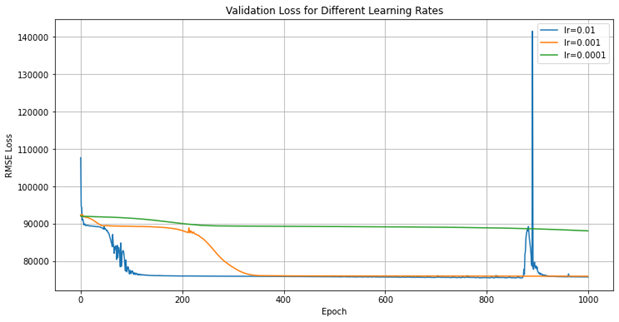
\includegraphics[width=0.8\textwidth]{image16.png}  % Adjust width as needed
   \caption{Validation loss across 1000 epochs for different learning rates: 0.01, 0.001, and 0.0001}
   \label{fig:brand_dist}
\end{figure}

\begin{figure}[H]
   \centering
   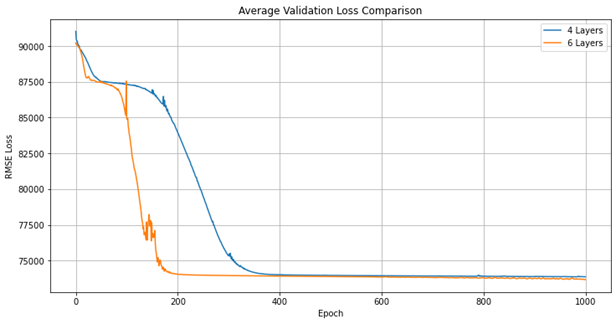
\includegraphics[width=0.8\textwidth]{image17.png}  % Adjust width as needed
   \caption{5-fold Average validation loss across 1000 epochs for different layers: 4 and 6}
   \label{fig:brand_dist}
\end{figure}

\begin{figure}[H]
   \centering
   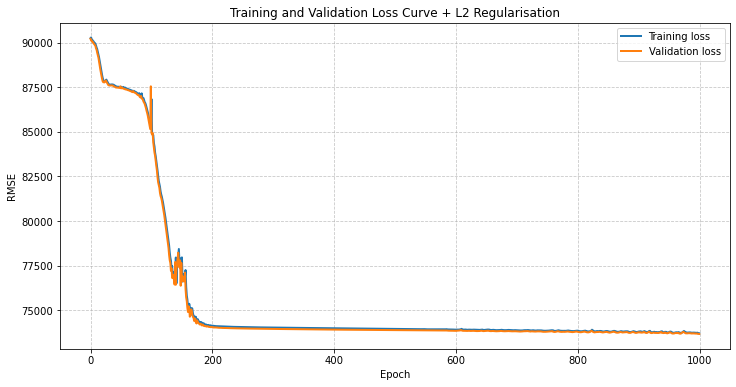
\includegraphics[width=0.8\textwidth]{image18.png}  % Adjust width as needed
   \caption{Training and validation losses for Model 6: 6 layers, learning rate: 0.001, with L2 regularization}
   \label{fig:brand_dist}
\end{figure}

\subsubsection{Gaussian Na\"{i}ve Bayes}

Gaussian Na\"{i}ve Bayes is a probabilistic classifier that extends Na\"{i}ve Bayes by assuming features follow a Gaussian distribution, chosen for our analysis since our target variable (\texttt{price}) and several features are continuous. Rather than discretizing continuous features through binning, which could lose discriminative information, we maintain their continuous nature by assuming Gaussian distributions. While this handles continuous data more appropriately, the fundamental Na\"{i}
ve Bayes assumption of conditional independence between features given the target variable remains.

\subsection{Training Procedure and Model Selection} 
The training of each model adheres to a consistent 5-fold cross-validation (CV) strategy to ensure robust performance evaluation. In this approach, the dataset is divided into five equal-sized folds. During each iteration, four folds are used for training while the remaining fold serves as the validation set. This process is repeated five times, ensuring that every fold is used as a validation set exactly once. The average Root Mean Squared Error (RMSE) across the five validation folds is computed to evaluate the model’s performance during training and hyperparameter tuning.

After the cross-validation process, each model is further evaluated on a held-out test set to calculate the test RMSE. This ensures that the model's performance is assessed on entirely unseen data, providing a reliable estimate of its generalization capability. For the final stage, the model with the best validation RMSE is re-trained on the entire training dataset (excluding the test set) to fully utilize all available data. This re-trained model is then used to generate final predictions on the test set, and the resulting RMSE is recorded as the model's definitive performance metric.  The consistency in training methodology across the Ridge Regression, LightGBM, XGBoost, CatBoost, and MLP models ensures fair comparisons, while the comprehensive use of CV and test evaluation provides a thorough assessment of each model’s predictive capability.

\section{Results and Discussion}

In this study, we aimed to predict car prices using machine learning models by leveraging a rich dataset of structured and unstructured features. Preprocessing was a critical component, involving the handling of missing values, extraction of information from unstructured text (e.g., engine and transmission details), and reducing the complexity of color variables by grouping nuanced tones into base color categories. These preprocessing steps ensured the dataset was clean, interpretable, and suitable for use in machine learning models. The models' performance was evaluated using both the 5-fold cross validation and the private leaderboard score on Kaggle, which calculates the RMSE on approximately 80\% of the unseen test data. The comparative results across models are presented in Table~6, and the actual Kaggle submission screenshots can be found in Appendix Figures~A.2 and~A.3.

\begin{table}[h!]
\centering
\caption{Comparison of Model Performance: 5-Fold Cross-Validation RMSE and Test Set Results.}
\begin{tabular}{lcc}
\toprule
\textbf{Model} & \textbf{Average RMSE across validation folds} & \textbf{RMSE on Test Set*} \\
\midrule
\textbf{LightGBM} & \textbf{72,806.06} & \textbf{63,481.83} \\
XGBoost & 73,235.15 & 63,671.16 \\
Catboost & 73,555.09 & 64,317.89 \\
Multi-Layer Perceptron & 73,665.02 & 64,529.35 \\
Gaussian Na\"{i}ve Bayes & 97,005.27 & 90,914.16 \\
\textbf{Ridge Regression} & \textbf{73,742.24} & \textbf{64,743.27} \\
\bottomrule
\end{tabular}
\begin{flushleft}
\footnotesize{\textit{*Test set consists of unseen data, and the predictions are evaluated through Kaggle's platform.}}
\end{flushleft}
\end{table}

Six machine learning models, ranging from simple regression to advanced gradient boosting and neural network models, were developed and compared. LightGBM emerged as the best-performing model, achieving the lowest RMSE on both validation and test sets. Its leaf-wise tree growth strategy, histogram-based learning, and ability to handle categorical variables natively allowed it to effectively model the complex, non-linear relationships in the dataset . Compared to Ridge Regression, which serves as a baseline linear model, LightGBM demonstrated superior performance, highlighting the need for more sophisticated algorithms to capture the nuances of car pricing.

The Multi-Layer Perceptron (MLP), a neural network model, exhibited a slightly higher RMSE compared to LightGBM, likely due to its increased sensitivity to hyperparameter tuning. While the current architecture does not exhibit overfitting, suggesting the potential for expanding the number of layers and nodes per layer, the performance could also be improved by incorporating additional features, such as learning rate scheduling. However, this would introduce more hyperparameters that require fine-tuning. Although these adjustments may reduce RMSE, they come with significantly higher computational resource demands and increase training duration compared to the more efficient tree-based models like LightGBM.

Gaussian Na\"{i}ve Bayes, on the other hand, exhibited the highest error due to its assumption of feature conditional independence, which is unrealistic for this dataset where variables like mileage, engine size, and year are highly correlated with price. This probabilistic approach also struggles with numerical and continuous features, leading to suboptimal performance.

A key limitation of this study was the highly skewed distribution of car prices, with a long tail of high-value cars. This right skewness likely introduced systemic errors, where models tended to underpredict prices for expensive cars and overpredict for cheaper ones. The RMSE metric, while useful for comparing overall model performance, may not fully capture these systemic errors, as it aggregates errors without distinguishing their directional biases. Future work could explore alternative metrics or loss functions (e.g., mean absolute percentage error) to better account for such biases ~\cite{Tofallis_2015}.

\section{Conclusion}

This study investigates the application of machine learning techniques for predicting resale prices of used cars, leveraging a comprehensive dataset comprising over 188,000 vehicle records. Following rigorous data preprocessing and feature engineering, six machine learning models were systematically evaluated. Among these, the LightGBM algorithm demonstrated superior performance, achieving a test root mean square error (RMSE) of 63,481.83, significantly outperforming the baseline Ridge Regression model (RMSE: 64,743.27). The results underscore the efficacy of advanced machine learning approaches in capturing the complexity of real-world car pricing data, characterized by non-linear relationships and intricate feature interactions. LightGBM's strengths in balancing accuracy, computational efficiency, and interpretability were particularly noteworthy. However, the study also highlights areas for further improvement, including addressing issues related to data skewness and prediction biases. These findings contribute to the growing body of research on automotive price prediction and demonstrate the practical utility of machine learning in addressing complex regression challenges.

\bibliographystyle{plain}
\bibliography{references}

\newpage

\appendix

\section{Appendix}

\renewcommand{\thetable}{A.\arabic{table}}
\setcounter{table}{0}
\begin{table}[h!]
  \centering
  \caption{Features in the dataset, source columns, derived columns, variable types, and characteristics}
  \begin{tabular}{lllcc}
      \toprule
      \textbf{Source} & \textbf{Column} & \textbf{Type} & \textbf{Levels} & \textbf{Dropped} \\
      \midrule
      id & \texttt{id} & numerical & -- & Yes \\
      model\_year & \texttt{model\_year} & numerical & -- & Yes \\
      milage & \texttt{milage} & numerical & -- & No \\
      accident & \texttt{accident} & categorical & 2 & No \\
      price & \texttt{price} & numerical & -- & No \\
      engine & \texttt{engine\_hp} & numerical & -- & No \\
      engine & \texttt{engine\_liter} & numerical & -- & No \\
      engine & \texttt{engine\_cyl} & numerical & -- & No \\
      transmission & \texttt{gears} & numerical & -- & No \\
      model\_year & \texttt{vehicle\_age} & numerical & -- & No \\
      brand & \texttt{is\_luxury\_brand} & categorical & 55 & No \\
      model & \texttt{model} & categorical & 1897 & Yes \\
      fuel\_type & \texttt{fuel\_type} & categorical & 6 & No \\
      engine & \texttt{engine} & categorical & 1117 & Yes \\
      transmission & \texttt{transmission} & categorical & 52 & Yes \\
      ext\_col & \texttt{ext\_col} & categorical & 15 & No \\
      int\_col & \texttt{int\_col} & categorical & 16 & No \\
      clean\_title & \texttt{clean\_title} & categorical & 2 & No \\
      engine & \texttt{engine\_fuel} & categorical & 6 & No \\
      transmission & \texttt{transmission\_type} & categorical & 6 & No \\
      transmission & \texttt{special\_features} & categorical & 6 & No \\
      transmission & \texttt{transmission\_designation} & categorical & 5 & No \\
      \bottomrule
  \end{tabular}
  \label{tab:features}
\end{table}

\renewcommand{\thefigure}{A.\arabic{figure}}  % Change figure numbering to A.1, A.2, etc.
\setcounter{figure}{1}  % Start counting from A.2

\begin{figure}[h!]
   \centering
   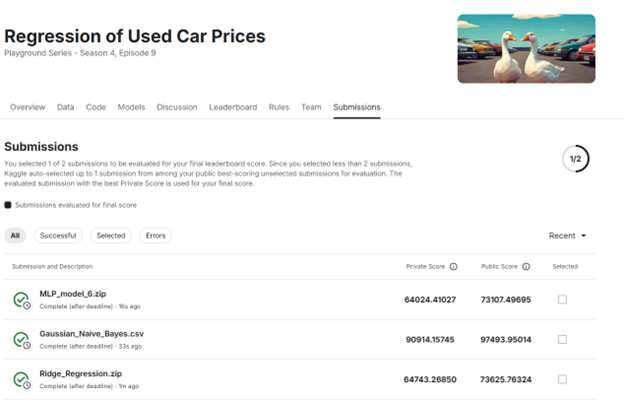
\includegraphics[width=0.8\textwidth]{image19.png}
   \caption{Screenshots for MLP, Gaussian a\"{i}ve Bayes and Ridge Regression}
   \label{fig:mlp_screenshot}
\end{figure}
\newpage
\begin{figure}[h!]
   \centering
   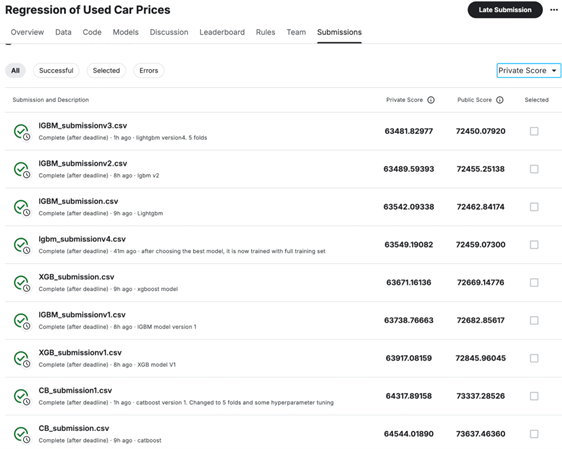
\includegraphics[width=0.8\textwidth]{image20.png}
   \caption{Screenshots for LGBM, XGB, and CB}
   \label{fig:boosting_screenshot}
\end{figure}

\end{document}